\documentclass[1p]{elsarticle_modified}
%\bibliographystyle{elsarticle-num}

%\usepackage[colorlinks]{hyperref}
%\usepackage{abbrmath_seonhwa} %\Abb, \Ascr, \Acal ,\Abf, \Afrak
\usepackage{amsfonts}
\usepackage{amssymb}
\usepackage{amsmath}
\usepackage{amsthm}
\usepackage{scalefnt}
\usepackage{amsbsy}
\usepackage{kotex}
\usepackage{caption}
\usepackage{subfig}
\usepackage{color}
\usepackage{graphicx}
\usepackage{xcolor} %% white, black, red, green, blue, cyan, magenta, yellow
\usepackage{float}
\usepackage{setspace}
\usepackage{hyperref}

\usepackage{tikz}
\usetikzlibrary{arrows}

\usepackage{multirow}
\usepackage{array} % fixed length table
\usepackage{hhline}

%%%%%%%%%%%%%%%%%%%%%
\makeatletter
\renewcommand*\env@matrix[1][\arraystretch]{%
	\edef\arraystretch{#1}%
	\hskip -\arraycolsep
	\let\@ifnextchar\new@ifnextchar
	\array{*\c@MaxMatrixCols c}}
\makeatother %https://tex.stackexchange.com/questions/14071/how-can-i-increase-the-line-spacing-in-a-matrix
%%%%%%%%%%%%%%%

\usepackage[normalem]{ulem}

\newcommand{\msout}[1]{\ifmmode\text{\sout{\ensuremath{#1}}}\else\sout{#1}\fi}
%SOURCE: \msout is \stkout macro in https://tex.stackexchange.com/questions/20609/strikeout-in-math-mode

\newcommand{\cancel}[1]{
	\ifmmode
	{\color{red}\msout{#1}}
	\else
	{\color{red}\sout{#1}}
	\fi
}

\newcommand{\add}[1]{
	{\color{blue}\uwave{#1}}
}

\newcommand{\replace}[2]{
	\ifmmode
	{\color{red}\msout{#1}}{\color{blue}\uwave{#2}}
	\else
	{\color{red}\sout{#1}}{\color{blue}\uwave{#2}}
	\fi
}

\newcommand{\Sol}{\mathcal{S}} %segment
\newcommand{\D}{D} %diagram
\newcommand{\A}{\mathcal{A}} %arc


%%%%%%%%%%%%%%%%%%%%%%%%%%%%%5 test

\def\sl{\operatorname{\textup{SL}}(2,\Cbb)}
\def\psl{\operatorname{\textup{PSL}}(2,\Cbb)}
\def\quan{\mkern 1mu \triangleright \mkern 1mu}

\theoremstyle{definition}
\newtheorem{thm}{Theorem}[section]
\newtheorem{prop}[thm]{Proposition}
\newtheorem{lem}[thm]{Lemma}
\newtheorem{ques}[thm]{Question}
\newtheorem{cor}[thm]{Corollary}
\newtheorem{defn}[thm]{Definition}
\newtheorem{exam}[thm]{Example}
\newtheorem{rmk}[thm]{Remark}
\newtheorem{alg}[thm]{Algorithm}

\newcommand{\I}{\sqrt{-1}}
\begin{document}

%\begin{frontmatter}
%
%\title{Boundary parabolic representations of knots up to 8 crossings}
%
%%% Group authors per affiliation:
%\author{Yunhi Cho} 
%\address{Department of Mathematics, University of Seoul, Seoul, Korea}
%\ead{yhcho@uos.ac.kr}
%
%
%\author{Seonhwa Kim} %\fnref{s_kim}}
%\address{Center for Geometry and Physics, Institute for Basic Science, Pohang, 37673, Korea}
%\ead{ryeona17@ibs.re.kr}
%
%\author{Hyuk Kim}
%\address{Department of Mathematical Sciences, Seoul National University, Seoul 08826, Korea}
%\ead{hyukkim@snu.ac.kr}
%
%\author{Seokbeom Yoon}
%\address{Department of Mathematical Sciences, Seoul National University, Seoul, 08826,  Korea}
%\ead{sbyoon15@snu.ac.kr}
%
%\begin{abstract}
%We find all boundary parabolic representation of knots up to 8 crossings.
%
%\end{abstract}
%\begin{keyword}
%    \MSC[2010] 57M25 
%\end{keyword}
%
%\end{frontmatter}

%\linenumbers
%\tableofcontents
%
\newcommand\colored[1]{\textcolor{white}{\rule[-0.35ex]{0.8em}{1.4ex}}\kern-0.8em\color{red} #1}%
%\newcommand\colored[1]{\textcolor{white}{ #1}\kern-2.17ex	\textcolor{white}{ #1}\kern-1.81ex	\textcolor{white}{ #1}\kern-2.15ex\color{red}#1	}

{\Large $\underline{11n_{166}~(K11n_{166})}$}

\setlength{\tabcolsep}{10pt}
\renewcommand{\arraystretch}{1.6}
\vspace{1cm}\begin{tabular}{m{100pt}>{\centering\arraybackslash}m{274pt}}
\multirow{5}{120pt}{
	\centering
	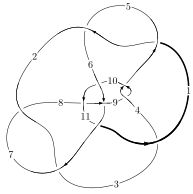
\includegraphics[width=112pt]{../../../GIT/diagram.site/Diagrams/png/782_11n_166.png}\\
\ \ \ A knot diagram\footnotemark}&
\allowdisplaybreaks
\textbf{Linearized knot diagam} \\
\cline{2-2}
 &
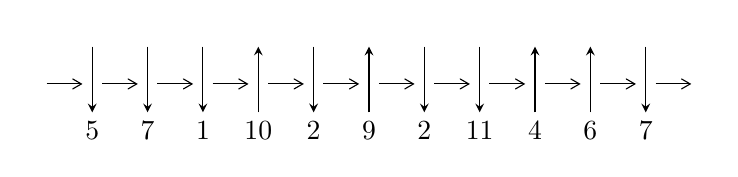
\begin{tikzpicture}[x=20pt, y=17pt]
	% nodes
	\node (C0) at (0, 0) {};
	\node (C1) at (1, 0) {};
	\node (C1U) at (1, +1) {};
	\node (C1D) at (1, -1) {5};

	\node (C2) at (2, 0) {};
	\node (C2U) at (2, +1) {};
	\node (C2D) at (2, -1) {7};

	\node (C3) at (3, 0) {};
	\node (C3U) at (3, +1) {};
	\node (C3D) at (3, -1) {1};

	\node (C4) at (4, 0) {};
	\node (C4U) at (4, +1) {};
	\node (C4D) at (4, -1) {10};

	\node (C5) at (5, 0) {};
	\node (C5U) at (5, +1) {};
	\node (C5D) at (5, -1) {2};

	\node (C6) at (6, 0) {};
	\node (C6U) at (6, +1) {};
	\node (C6D) at (6, -1) {9};

	\node (C7) at (7, 0) {};
	\node (C7U) at (7, +1) {};
	\node (C7D) at (7, -1) {2};

	\node (C8) at (8, 0) {};
	\node (C8U) at (8, +1) {};
	\node (C8D) at (8, -1) {11};

	\node (C9) at (9, 0) {};
	\node (C9U) at (9, +1) {};
	\node (C9D) at (9, -1) {4};

	\node (C10) at (10, 0) {};
	\node (C10U) at (10, +1) {};
	\node (C10D) at (10, -1) {6};

	\node (C11) at (11, 0) {};
	\node (C11U) at (11, +1) {};
	\node (C11D) at (11, -1) {7};
	\node (C12) at (12, 0) {};

	% arrows
	\draw[->,>={angle 60}]
	(C0) edge (C1) (C1) edge (C2) (C2) edge (C3) (C3) edge (C4) (C4) edge (C5) (C5) edge (C6) (C6) edge (C7) (C7) edge (C8) (C8) edge (C9) (C9) edge (C10) (C10) edge (C11) (C11) edge (C12) ;	\draw[->,>=stealth]
	(C1U) edge (C1D) (C2U) edge (C2D) (C3U) edge (C3D) (C4D) edge (C4U) (C5U) edge (C5D) (C6D) edge (C6U) (C7U) edge (C7D) (C8U) edge (C8D) (C9D) edge (C9U) (C10D) edge (C10U) (C11U) edge (C11D) ;
	\end{tikzpicture} \\
\hhline{~~} \\& 
\textbf{Solving Sequence} \\ \cline{2-2} 
 &
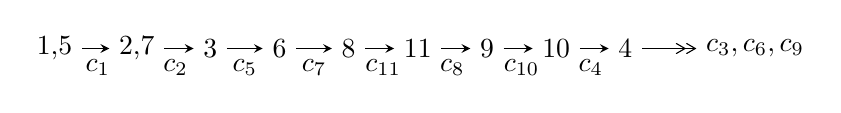
\begin{tikzpicture}[x=25pt, y=7pt]
	% node
	\node (A0) at (-1/8, 0) {1,5};
	\node (A1) at (17/16, 0) {2,7};
	\node (A2) at (17/8, 0) {3};
	\node (A3) at (25/8, 0) {6};
	\node (A4) at (33/8, 0) {8};
	\node (A5) at (41/8, 0) {11};
	\node (A6) at (49/8, 0) {9};
	\node (A7) at (57/8, 0) {10};
	\node (A8) at (65/8, 0) {4};
	\node (C1) at (1/2, -1) {$c_{1}$};
	\node (C2) at (13/8, -1) {$c_{2}$};
	\node (C3) at (21/8, -1) {$c_{5}$};
	\node (C4) at (29/8, -1) {$c_{7}$};
	\node (C5) at (37/8, -1) {$c_{11}$};
	\node (C6) at (45/8, -1) {$c_{8}$};
	\node (C7) at (53/8, -1) {$c_{10}$};
	\node (C8) at (61/8, -1) {$c_{4}$};
	\node (A9) at (10, 0) {$c_{3},c_{6},c_{9}$};

	% edge
	\draw[->,>=stealth]	
	(A0) edge (A1) (A1) edge (A2) (A2) edge (A3) (A3) edge (A4) (A4) edge (A5) (A5) edge (A6) (A6) edge (A7) (A7) edge (A8) ;
	\draw[->>,>={angle 60}]	
	(A8) edge (A9);
\end{tikzpicture} \\ 

\end{tabular} \\

\footnotetext{
The image of knot diagram is generated by the software ``\textbf{Draw programme}" developed by Andrew Bartholomew(\url{http://www.layer8.co.uk/maths/draw/index.htm\#Running-draw}), where we modified some parts for our purpose(\url{https://github.com/CATsTAILs/LinksPainter}).
}\phantom \\ \newline 
\centering \textbf{Ideals for irreducible components\footnotemark of $X_{\text{par}}$} 
 
\begin{align*}
I^u_{1}&=\langle 
1.30687\times10^{68} u^{41}-1.54062\times10^{68} u^{40}+\cdots+9.86366\times10^{67} b+1.76058\times10^{68},\\
\phantom{I^u_{1}}&\phantom{= \langle  }-2.28329\times10^{67} u^{41}-9.73388\times10^{67} u^{40}+\cdots+9.86366\times10^{67} a+5.08435\times10^{68},\\
\phantom{I^u_{1}}&\phantom{= \langle  }u^{42}-2 u^{41}+\cdots-12 u-1\rangle \\
I^u_{2}&=\langle 
-33 u^{12}-73 u^{11}+\cdots+23 b-41,\;-242 u^{12}-589 u^{11}+\cdots+23 a-362,\\
\phantom{I^u_{2}}&\phantom{= \langle  }u^{13}+3 u^{12}+2 u^{11}-3 u^{10}-9 u^9-9 u^8+5 u^7+18 u^6+7 u^5-9 u^4-9 u^3+3 u+1\rangle \\
\\
\end{align*}
\raggedright * 2 irreducible components of $\dim_{\mathbb{C}}=0$, with total 55 representations.\\
\footnotetext{All coefficients of polynomials are rational numbers. But the coefficients are sometimes approximated in decimal forms when there is not enough margin.}
\newpage
\renewcommand{\arraystretch}{1}
\centering \section*{I. $I^u_{1}= \langle 1.31\times10^{68} u^{41}-1.54\times10^{68} u^{40}+\cdots+9.86\times10^{67} b+1.76\times10^{68},\;-2.28\times10^{67} u^{41}-9.73\times10^{67} u^{40}+\cdots+9.86\times10^{67} a+5.08\times10^{68},\;u^{42}-2 u^{41}+\cdots-12 u-1 \rangle$}
\flushleft \textbf{(i) Arc colorings}\\
\begin{tabular}{m{7pt} m{180pt} m{7pt} m{180pt} }
\flushright $a_{1}=$&$\begin{pmatrix}1\\0\end{pmatrix}$ \\
\flushright $a_{5}=$&$\begin{pmatrix}0\\u\end{pmatrix}$ \\
\flushright $a_{2}=$&$\begin{pmatrix}1\\u^2\end{pmatrix}$ \\
\flushright $a_{7}=$&$\begin{pmatrix}0.231485 u^{41}+0.986842 u^{40}+\cdots+194.921 u-5.15463\\-1.32493 u^{41}+1.56192 u^{40}+\cdots-20.7796 u-1.78491\end{pmatrix}$ \\
\flushright $a_{3}=$&$\begin{pmatrix}5.28014 u^{41}-6.60175 u^{40}+\cdots+194.483 u+34.5032\\-0.411012 u^{41}+0.388919 u^{40}+\cdots-0.134181 u-0.550999\end{pmatrix}$ \\
\flushright $a_{6}=$&$\begin{pmatrix}- u\\- u^3+u\end{pmatrix}$ \\
\flushright $a_{8}=$&$\begin{pmatrix}2.74943 u^{41}-1.78847 u^{40}+\cdots+233.329 u-1.91990\\0.549437 u^{41}-0.604447 u^{40}+\cdots+8.86516 u+0.475658\end{pmatrix}$ \\
\flushright $a_{11}=$&$\begin{pmatrix}-3.86650 u^{41}+4.37940 u^{40}+\cdots-154.682 u-24.8689\\-1.84296 u^{41}+2.51664 u^{40}+\cdots-43.9754 u-2.80259\end{pmatrix}$ \\
\flushright $a_{9}=$&$\begin{pmatrix}-10.3413 u^{41}+13.9461 u^{40}+\cdots-201.572 u-32.5039\\7.39043 u^{41}-10.4148 u^{40}+\cdots+159.817 u+12.0772\end{pmatrix}$ \\
\flushright $a_{10}=$&$\begin{pmatrix}-2.07285 u^{41}+1.91194 u^{40}+\cdots-116.180 u-21.9484\\-2.88801 u^{41}+4.05483 u^{40}+\cdots-67.2450 u-4.60324\end{pmatrix}$ \\
\flushright $a_{4}=$&$\begin{pmatrix}5.69115 u^{41}-6.99067 u^{40}+\cdots+194.617 u+35.0542\\-0.411012 u^{41}+0.388919 u^{40}+\cdots-0.134181 u-0.550999\end{pmatrix}$\\ \flushright $a_{4}=$&$\begin{pmatrix}5.69115 u^{41}-6.99067 u^{40}+\cdots+194.617 u+35.0542\\-0.411012 u^{41}+0.388919 u^{40}+\cdots-0.134181 u-0.550999\end{pmatrix}$\\&\end{tabular}
\flushleft \textbf{(ii) Obstruction class $= -1$}\\~\\
\flushleft \textbf{(iii) Cusp Shapes $= 29.0951 u^{41}-41.2441 u^{40}+\cdots+827.490 u+68.4277$}\\~\\
\newpage\renewcommand{\arraystretch}{1}
\flushleft \textbf{(iv) u-Polynomials at the component}\newline \\
\begin{tabular}{m{50pt}|m{274pt}}
Crossings & \hspace{64pt}u-Polynomials at each crossing \\
\hline $$\begin{aligned}c_{1},c_{5}\end{aligned}$$&$\begin{aligned}
&u^{42}+2 u^{41}+\cdots+12 u-1
\end{aligned}$\\
\hline $$\begin{aligned}c_{2},c_{7}\end{aligned}$$&$\begin{aligned}
&u^{42}+u^{41}+\cdots+29 u+151
\end{aligned}$\\
\hline $$\begin{aligned}c_{3}\end{aligned}$$&$\begin{aligned}
&u^{42}-3 u^{41}+\cdots+75 u+19
\end{aligned}$\\
\hline $$\begin{aligned}c_{4},c_{9}\end{aligned}$$&$\begin{aligned}
&u^{42}+3 u^{41}+\cdots+21 u+13
\end{aligned}$\\
\hline $$\begin{aligned}c_{6}\end{aligned}$$&$\begin{aligned}
&u^{42}+6 u^{41}+\cdots+15 u+1
\end{aligned}$\\
\hline $$\begin{aligned}c_{8}\end{aligned}$$&$\begin{aligned}
&u^{42}-6 u^{41}+\cdots-87352 u+17077
\end{aligned}$\\
\hline $$\begin{aligned}c_{10}\end{aligned}$$&$\begin{aligned}
&u^{42}-2 u^{41}+\cdots-423 u-43
\end{aligned}$\\
\hline $$\begin{aligned}c_{11}\end{aligned}$$&$\begin{aligned}
&u^{42}+u^{41}+\cdots+2205 u+297
\end{aligned}$\\
\hline
\end{tabular}\\~\\
\newpage\renewcommand{\arraystretch}{1}
\flushleft \textbf{(v) Riley Polynomials at the component}\newline \\
\begin{tabular}{m{50pt}|m{274pt}}
Crossings & \hspace{64pt}Riley Polynomials at each crossing \\
\hline $$\begin{aligned}c_{1},c_{5}\end{aligned}$$&$\begin{aligned}
&y^{42}-30 y^{41}+\cdots-44 y+1
\end{aligned}$\\
\hline $$\begin{aligned}c_{2},c_{7}\end{aligned}$$&$\begin{aligned}
&y^{42}-57 y^{41}+\cdots-202275 y+22801
\end{aligned}$\\
\hline $$\begin{aligned}c_{3}\end{aligned}$$&$\begin{aligned}
&y^{42}-61 y^{41}+\cdots-7753 y+361
\end{aligned}$\\
\hline $$\begin{aligned}c_{4},c_{9}\end{aligned}$$&$\begin{aligned}
&y^{42}-25 y^{41}+\cdots-2261 y+169
\end{aligned}$\\
\hline $$\begin{aligned}c_{6}\end{aligned}$$&$\begin{aligned}
&y^{42}-2 y^{41}+\cdots-9 y+1
\end{aligned}$\\
\hline $$\begin{aligned}c_{8}\end{aligned}$$&$\begin{aligned}
&y^{42}-58 y^{41}+\cdots-2530360008 y+291623929
\end{aligned}$\\
\hline $$\begin{aligned}c_{10}\end{aligned}$$&$\begin{aligned}
&y^{42}+10 y^{41}+\cdots+9411 y+1849
\end{aligned}$\\
\hline $$\begin{aligned}c_{11}\end{aligned}$$&$\begin{aligned}
&y^{42}-57 y^{41}+\cdots-501471 y+88209
\end{aligned}$\\
\hline
\end{tabular}\\~\\
\newpage\flushleft \textbf{(vi) Complex Volumes and Cusp Shapes}
$$\begin{array}{c|c|c}  
\text{Solutions to }I^u_{1}& \I (\text{vol} + \sqrt{-1}CS) & \text{Cusp shape}\\
 \hline 
\begin{aligned}
u &= \phantom{-}0.971644 + 0.228980 I \\
a &= -0.660225 - 0.077093 I \\
b &= \phantom{-}0.121229 - 0.121842 I\end{aligned}
 & -1.74908 - 0.43337 I & -4.63201 + 0.76425 I \\ \hline\begin{aligned}
u &= \phantom{-}0.971644 - 0.228980 I \\
a &= -0.660225 + 0.077093 I \\
b &= \phantom{-}0.121229 + 0.121842 I\end{aligned}
 & -1.74908 + 0.43337 I & -4.63201 - 0.76425 I \\ \hline\begin{aligned}
u &= -0.935799 + 0.492680 I \\
a &= \phantom{-}0.995156 + 0.254691 I \\
b &= \phantom{-}0.697241 - 0.562142 I\end{aligned}
 & -1.54069 + 4.15417 I & -3.00000 - 7.39011 I \\ \hline\begin{aligned}
u &= -0.935799 - 0.492680 I \\
a &= \phantom{-}0.995156 - 0.254691 I \\
b &= \phantom{-}0.697241 + 0.562142 I\end{aligned}
 & -1.54069 - 4.15417 I & -3.00000 + 7.39011 I \\ \hline\begin{aligned}
u &= -0.393155 + 0.800612 I \\
a &= -0.149356 - 0.205071 I \\
b &= -0.541363 + 0.329653 I\end{aligned}
 & \phantom{-}2.76017 - 1.64933 I & -1.74728 + 0.60366 I \\ \hline\begin{aligned}
u &= -0.393155 - 0.800612 I \\
a &= -0.149356 + 0.205071 I \\
b &= -0.541363 - 0.329653 I\end{aligned}
 & \phantom{-}2.76017 + 1.64933 I & -1.74728 - 0.60366 I \\ \hline\begin{aligned}
u &= \phantom{-}1.104400 + 0.249694 I \\
a &= \phantom{-}0.436118 - 0.996945 I \\
b &= \phantom{-}0.530412 + 0.326797 I\end{aligned}
 & -2.78567 - 0.99125 I & -11.10311 - 4.39500 I \\ \hline\begin{aligned}
u &= \phantom{-}1.104400 - 0.249694 I \\
a &= \phantom{-}0.436118 + 0.996945 I \\
b &= \phantom{-}0.530412 - 0.326797 I\end{aligned}
 & -2.78567 + 0.99125 I & -11.10311 + 4.39500 I \\ \hline\begin{aligned}
u &= -1.155180 + 0.226642 I \\
a &= \phantom{-}0.752466 + 0.511395 I \\
b &= \phantom{-}0.896926 + 1.040480 I\end{aligned}
 & -1.88826 - 1.20315 I & \phantom{-0.000000 } 0 \\ \hline\begin{aligned}
u &= -1.155180 - 0.226642 I \\
a &= \phantom{-}0.752466 - 0.511395 I \\
b &= \phantom{-}0.896926 - 1.040480 I\end{aligned}
 & -1.88826 + 1.20315 I & \phantom{-0.000000 } 0\\
 \hline 
 \end{array}$$\newpage$$\begin{array}{c|c|c}  
\text{Solutions to }I^u_{1}& \I (\text{vol} + \sqrt{-1}CS) & \text{Cusp shape}\\
 \hline 
\begin{aligned}
u &= \phantom{-}1.17730\phantom{ +0.000000I} \\
a &= \phantom{-}2.81430\phantom{ +0.000000I} \\
b &= \phantom{-}1.42191\phantom{ +0.000000I}\end{aligned}
 & -4.47617\phantom{ +0.000000I} & \phantom{-}5.20530\phantom{ +0.000000I} \\ \hline\begin{aligned}
u &= \phantom{-}1.255780 + 0.019663 I \\
a &= -2.27463 - 0.18547 I \\
b &= -1.95961 - 0.66957 I\end{aligned}
 & -7.36750 - 2.87143 I & \phantom{-0.000000 } 0 \\ \hline\begin{aligned}
u &= \phantom{-}1.255780 - 0.019663 I \\
a &= -2.27463 + 0.18547 I \\
b &= -1.95961 + 0.66957 I\end{aligned}
 & -7.36750 + 2.87143 I & \phantom{-0.000000 } 0 \\ \hline\begin{aligned}
u &= -1.114120 + 0.594857 I \\
a &= -0.017502 - 0.611763 I \\
b &= -0.609070 - 0.365005 I\end{aligned}
 & \phantom{-}0.58975 + 6.86368 I & \phantom{-0.000000 } 0 \\ \hline\begin{aligned}
u &= -1.114120 - 0.594857 I \\
a &= -0.017502 + 0.611763 I \\
b &= -0.609070 + 0.365005 I\end{aligned}
 & \phantom{-}0.58975 - 6.86368 I & \phantom{-0.000000 } 0 \\ \hline\begin{aligned}
u &= \phantom{-}0.514470 + 1.177460 I \\
a &= -0.0735393 - 0.0954487 I \\
b &= -1.57588 + 0.26064 I\end{aligned}
 & -5.82264 - 2.10553 I & \phantom{-0.000000 } 0 \\ \hline\begin{aligned}
u &= \phantom{-}0.514470 - 1.177460 I \\
a &= -0.0735393 + 0.0954487 I \\
b &= -1.57588 - 0.26064 I\end{aligned}
 & -5.82264 + 2.10553 I & \phantom{-0.000000 } 0 \\ \hline\begin{aligned}
u &= -1.367560 + 0.254517 I \\
a &= -0.890031 + 0.144472 I \\
b &= -0.850798 - 0.662707 I\end{aligned}
 & -0.09515 + 5.56736 I & \phantom{-0.000000 } 0 \\ \hline\begin{aligned}
u &= -1.367560 - 0.254517 I \\
a &= -0.890031 - 0.144472 I \\
b &= -0.850798 + 0.662707 I\end{aligned}
 & -0.09515 - 5.56736 I & \phantom{-0.000000 } 0 \\ \hline\begin{aligned}
u &= \phantom{-}0.574212 + 0.117339 I \\
a &= -0.393410 - 0.999550 I \\
b &= -1.252340 - 0.394572 I\end{aligned}
 & -4.70197 - 3.01261 I & -11.65660 + 2.21081 I\\
 \hline 
 \end{array}$$\newpage$$\begin{array}{c|c|c}  
\text{Solutions to }I^u_{1}& \I (\text{vol} + \sqrt{-1}CS) & \text{Cusp shape}\\
 \hline 
\begin{aligned}
u &= \phantom{-}0.574212 - 0.117339 I \\
a &= -0.393410 + 0.999550 I \\
b &= -1.252340 + 0.394572 I\end{aligned}
 & -4.70197 + 3.01261 I & -11.65660 - 2.21081 I \\ \hline\begin{aligned}
u &= \phantom{-}0.568925 + 0.051008 I \\
a &= -1.46927 - 0.44701 I \\
b &= \phantom{-}1.069300 - 0.013204 I\end{aligned}
 & -2.53352 - 0.05674 I & -5.88497 - 7.01523 I \\ \hline\begin{aligned}
u &= \phantom{-}0.568925 - 0.051008 I \\
a &= -1.46927 + 0.44701 I \\
b &= \phantom{-}1.069300 + 0.013204 I\end{aligned}
 & -2.53352 + 0.05674 I & -5.88497 + 7.01523 I \\ \hline\begin{aligned}
u &= -0.07204 + 1.42728 I \\
a &= -0.086850 - 1.160690 I \\
b &= -0.345695 + 1.176360 I\end{aligned}
 & \phantom{-}5.55360 - 0.39636 I & \phantom{-0.000000 } 0 \\ \hline\begin{aligned}
u &= -0.07204 - 1.42728 I \\
a &= -0.086850 + 1.160690 I \\
b &= -0.345695 - 1.176360 I\end{aligned}
 & \phantom{-}5.55360 + 0.39636 I & \phantom{-0.000000 } 0 \\ \hline\begin{aligned}
u &= \phantom{-}1.48422 + 0.23506 I \\
a &= -0.717440 - 0.244330 I \\
b &= -0.52362 - 1.68426 I\end{aligned}
 & -1.15694 - 4.97445 I & \phantom{-0.000000 } 0 \\ \hline\begin{aligned}
u &= \phantom{-}1.48422 - 0.23506 I \\
a &= -0.717440 + 0.244330 I \\
b &= -0.52362 + 1.68426 I\end{aligned}
 & -1.15694 + 4.97445 I & \phantom{-0.000000 } 0 \\ \hline\begin{aligned}
u &= \phantom{-}0.11486 + 1.51372 I \\
a &= -0.0321052 + 0.0488945 I \\
b &= \phantom{-}2.03791 - 0.23200 I\end{aligned}
 & -4.38173 + 6.68735 I & \phantom{-0.000000 } 0 \\ \hline\begin{aligned}
u &= \phantom{-}0.11486 - 1.51372 I \\
a &= -0.0321052 - 0.0488945 I \\
b &= \phantom{-}2.03791 + 0.23200 I\end{aligned}
 & -4.38173 - 6.68735 I & \phantom{-0.000000 } 0 \\ \hline\begin{aligned}
u &= -1.47470 + 0.37744 I \\
a &= -1.67468 - 0.56566 I \\
b &= -1.90596 + 0.26710 I\end{aligned}
 & -12.10630 + 7.14794 I & \phantom{-0.000000 } 0\\
 \hline 
 \end{array}$$\newpage$$\begin{array}{c|c|c}  
\text{Solutions to }I^u_{1}& \I (\text{vol} + \sqrt{-1}CS) & \text{Cusp shape}\\
 \hline 
\begin{aligned}
u &= -1.47470 - 0.37744 I \\
a &= -1.67468 + 0.56566 I \\
b &= -1.90596 - 0.26710 I\end{aligned}
 & -12.10630 - 7.14794 I & \phantom{-0.000000 } 0 \\ \hline\begin{aligned}
u &= -1.62716\phantom{ +0.000000I} \\
a &= \phantom{-}1.69579\phantom{ +0.000000I} \\
b &= \phantom{-}2.74174\phantom{ +0.000000I}\end{aligned}
 & -10.4541\phantom{ +0.000000I} & \phantom{-0.000000 } 0 \\ \hline\begin{aligned}
u &= \phantom{-}1.48967 + 0.67284 I \\
a &= \phantom{-}1.32309 - 0.83780 I \\
b &= \phantom{-}1.98195 + 0.65769 I\end{aligned}
 & -8.8694 - 14.1954 I & \phantom{-0.000000 } 0 \\ \hline\begin{aligned}
u &= \phantom{-}1.48967 - 0.67284 I \\
a &= \phantom{-}1.32309 + 0.83780 I \\
b &= \phantom{-}1.98195 - 0.65769 I\end{aligned}
 & -8.8694 + 14.1954 I & \phantom{-0.000000 } 0 \\ \hline\begin{aligned}
u &= \phantom{-}1.45552 + 0.81312 I \\
a &= -1.080210 + 0.896892 I \\
b &= -1.75516 - 0.59909 I\end{aligned}
 & -8.67069 - 5.62021 I & \phantom{-0.000000 } 0 \\ \hline\begin{aligned}
u &= \phantom{-}1.45552 - 0.81312 I \\
a &= -1.080210 - 0.896892 I \\
b &= -1.75516 + 0.59909 I\end{aligned}
 & -8.67069 + 5.62021 I & \phantom{-0.000000 } 0 \\ \hline\begin{aligned}
u &= -0.049563 + 0.302088 I \\
a &= -1.34651 + 0.47011 I \\
b &= \phantom{-}0.315782 + 0.486715 I\end{aligned}
 & -0.096362 - 1.232180 I & -1.37808 + 5.47691 I \\ \hline\begin{aligned}
u &= -0.049563 - 0.302088 I \\
a &= -1.34651 - 0.47011 I \\
b &= \phantom{-}0.315782 - 0.486715 I\end{aligned}
 & -0.096362 + 1.232180 I & -1.37808 - 5.47691 I \\ \hline\begin{aligned}
u &= -1.68157 + 0.33743 I \\
a &= \phantom{-}1.39696 + 0.40870 I \\
b &= \phantom{-}2.25961 - 0.16660 I\end{aligned}
 & -11.08320 + 0.67325 I & \phantom{-0.000000 } 0 \\ \hline\begin{aligned}
u &= -1.68157 - 0.33743 I \\
a &= \phantom{-}1.39696 - 0.40870 I \\
b &= \phantom{-}2.25961 + 0.16660 I\end{aligned}
 & -11.08320 - 0.67325 I & \phantom{-0.000000 } 0\\
 \hline 
 \end{array}$$\newpage$$\begin{array}{c|c|c}  
\text{Solutions to }I^u_{1}& \I (\text{vol} + \sqrt{-1}CS) & \text{Cusp shape}\\
 \hline 
\begin{aligned}
u &= -0.0650964 + 0.0552947 I \\
a &= -17.7931 + 18.4218 I \\
b &= -0.172689 - 0.653820 I\end{aligned}
 & \phantom{-}5.14610 - 3.90439 I & \phantom{-}9.21708 + 9.57987 I \\ \hline\begin{aligned}
u &= -0.0650964 - 0.0552947 I \\
a &= -17.7931 - 18.4218 I \\
b &= -0.172689 + 0.653820 I\end{aligned}
 & \phantom{-}5.14610 + 3.90439 I & \phantom{-}9.21708 - 9.57987 I\\
 \hline 
 \end{array}$$\newpage\newpage\renewcommand{\arraystretch}{1}
\centering \section*{II. $I^u_{2}= \langle -33 u^{12}-73 u^{11}+\cdots+23 b-41,\;-242 u^{12}-589 u^{11}+\cdots+23 a-362,\;u^{13}+3 u^{12}+\cdots+3 u+1 \rangle$}
\flushleft \textbf{(i) Arc colorings}\\
\begin{tabular}{m{7pt} m{180pt} m{7pt} m{180pt} }
\flushright $a_{1}=$&$\begin{pmatrix}1\\0\end{pmatrix}$ \\
\flushright $a_{5}=$&$\begin{pmatrix}0\\u\end{pmatrix}$ \\
\flushright $a_{2}=$&$\begin{pmatrix}1\\u^2\end{pmatrix}$ \\
\flushright $a_{7}=$&$\begin{pmatrix}10.5217 u^{12}+25.6087 u^{11}+\cdots+23.0870 u+15.7391\\1.43478 u^{12}+3.17391 u^{11}+\cdots+1.73913 u+1.78261\end{pmatrix}$ \\
\flushright $a_{3}=$&$\begin{pmatrix}-2.26087 u^{12}-5.30435 u^{11}+\cdots-3.04348 u+2.13043\\-0.695652 u^{12}-1.47826 u^{11}+\cdots-3.78261 u-1.65217\end{pmatrix}$ \\
\flushright $a_{6}=$&$\begin{pmatrix}- u\\- u^3+u\end{pmatrix}$ \\
\flushright $a_{8}=$&$\begin{pmatrix}13.1739 u^{12}+32.8696 u^{11}+\cdots+28.6957 u+19.9130\\2.04348 u^{12}+5.21739 u^{11}+\cdots+1.17391 u+2.47826\end{pmatrix}$ \\
\flushright $a_{11}=$&$\begin{pmatrix}0.521739 u^{12}+2.60870 u^{11}+\cdots+0.0869565 u+3.73913\\-0.217391 u^{12}-0.0869565 u^{11}+\cdots+0.130435 u+0.608696\end{pmatrix}$ \\
\flushright $a_{9}=$&$\begin{pmatrix}2.04348 u^{12}+2.21739 u^{11}+\cdots+18.1739 u+5.47826\\1.73913 u^{12}+5.69565 u^{11}+\cdots-2.04348 u+1.13043\end{pmatrix}$ \\
\flushright $a_{10}=$&$\begin{pmatrix}1.65217 u^{12}+5.26087 u^{11}+\cdots+2.60870 u+4.17391\\-0.826087 u^{12}-1.13043 u^{11}+\cdots-1.30435 u+0.913043\end{pmatrix}$ \\
\flushright $a_{4}=$&$\begin{pmatrix}-1.56522 u^{12}-3.82609 u^{11}+\cdots+0.739130 u+3.78261\\-0.695652 u^{12}-1.47826 u^{11}+\cdots-3.78261 u-1.65217\end{pmatrix}$\\ \flushright $a_{4}=$&$\begin{pmatrix}-1.56522 u^{12}-3.82609 u^{11}+\cdots+0.739130 u+3.78261\\-0.695652 u^{12}-1.47826 u^{11}+\cdots-3.78261 u-1.65217\end{pmatrix}$\\&\end{tabular}
\flushleft \textbf{(ii) Obstruction class $= 1$}\\~\\
\flushleft \textbf{(iii) Cusp Shapes $= \frac{15}{23} u^{12}-\frac{17}{23} u^{11}-\frac{142}{23} u^{10}-\frac{214}{23} u^9-\frac{218}{23} u^8+\frac{27}{23} u^7+\frac{451}{23} u^6+\frac{459}{23} u^5+\frac{195}{23} u^4+\frac{117}{23} u^3-\frac{246}{23} u^2-\frac{492}{23} u-\frac{387}{23}$}\\~\\
\newpage\renewcommand{\arraystretch}{1}
\flushleft \textbf{(iv) u-Polynomials at the component}\newline \\
\begin{tabular}{m{50pt}|m{274pt}}
Crossings & \hspace{64pt}u-Polynomials at each crossing \\
\hline $$\begin{aligned}c_{1}\end{aligned}$$&$\begin{aligned}
&u^{13}+3 u^{12}+\cdots+3 u+1
\end{aligned}$\\
\hline $$\begin{aligned}c_{2}\end{aligned}$$&$\begin{aligned}
&u^{13}+2 u^{12}+\cdots-2 u+1
\end{aligned}$\\
\hline $$\begin{aligned}c_{3}\end{aligned}$$&$\begin{aligned}
&u^{13}+8 u^{12}+\cdots-46 u-11
\end{aligned}$\\
\hline $$\begin{aligned}c_{4}\end{aligned}$$&$\begin{aligned}
&u^{13}+2 u^{12}+\cdots-2 u-1
\end{aligned}$\\
\hline $$\begin{aligned}c_{5}\end{aligned}$$&$\begin{aligned}
&u^{13}-3 u^{12}+\cdots+3 u-1
\end{aligned}$\\
\hline $$\begin{aligned}c_{6}\end{aligned}$$&$\begin{aligned}
&u^{13}+7 u^{12}+\cdots-2 u-1
\end{aligned}$\\
\hline $$\begin{aligned}c_{7}\end{aligned}$$&$\begin{aligned}
&u^{13}-2 u^{12}+\cdots-2 u-1
\end{aligned}$\\
\hline $$\begin{aligned}c_{8}\end{aligned}$$&$\begin{aligned}
&u^{13}+u^{12}+\cdots- u-1
\end{aligned}$\\
\hline $$\begin{aligned}c_{9}\end{aligned}$$&$\begin{aligned}
&u^{13}-2 u^{12}+\cdots-2 u+1
\end{aligned}$\\
\hline $$\begin{aligned}c_{10}\end{aligned}$$&$\begin{aligned}
&u^{13}+u^{12}+\cdots+2 u-1
\end{aligned}$\\
\hline $$\begin{aligned}c_{11}\end{aligned}$$&$\begin{aligned}
&u^{13}-2 u^{12}+\cdots-2 u-1
\end{aligned}$\\
\hline
\end{tabular}\\~\\
\newpage\renewcommand{\arraystretch}{1}
\flushleft \textbf{(v) Riley Polynomials at the component}\newline \\
\begin{tabular}{m{50pt}|m{274pt}}
Crossings & \hspace{64pt}Riley Polynomials at each crossing \\
\hline $$\begin{aligned}c_{1},c_{5}\end{aligned}$$&$\begin{aligned}
&y^{13}-5 y^{12}+\cdots+9 y-1
\end{aligned}$\\
\hline $$\begin{aligned}c_{2},c_{7}\end{aligned}$$&$\begin{aligned}
&y^{13}-4 y^{12}+\cdots-8 y-1
\end{aligned}$\\
\hline $$\begin{aligned}c_{3}\end{aligned}$$&$\begin{aligned}
&y^{13}-16 y^{12}+\cdots+774 y-121
\end{aligned}$\\
\hline $$\begin{aligned}c_{4},c_{9}\end{aligned}$$&$\begin{aligned}
&y^{13}-12 y^{12}+\cdots+2 y-1
\end{aligned}$\\
\hline $$\begin{aligned}c_{6}\end{aligned}$$&$\begin{aligned}
&y^{13}-5 y^{12}+\cdots-10 y-1
\end{aligned}$\\
\hline $$\begin{aligned}c_{8}\end{aligned}$$&$\begin{aligned}
&y^{13}+11 y^{12}+\cdots-7 y-1
\end{aligned}$\\
\hline $$\begin{aligned}c_{10}\end{aligned}$$&$\begin{aligned}
&y^{13}-5 y^{12}+\cdots+2 y-1
\end{aligned}$\\
\hline $$\begin{aligned}c_{11}\end{aligned}$$&$\begin{aligned}
&y^{13}-8 y^{12}+\cdots-8 y-1
\end{aligned}$\\
\hline
\end{tabular}\\~\\
\newpage\flushleft \textbf{(vi) Complex Volumes and Cusp Shapes}
$$\begin{array}{c|c|c}  
\text{Solutions to }I^u_{2}& \I (\text{vol} + \sqrt{-1}CS) & \text{Cusp shape}\\
 \hline 
\begin{aligned}
u &= \phantom{-}1.059650 + 0.184275 I \\
a &= -0.698885 - 0.288098 I \\
b &= -0.410177 - 0.918523 I\end{aligned}
 & -1.83033 - 2.41287 I & -3.84698 + 4.49416 I \\ \hline\begin{aligned}
u &= \phantom{-}1.059650 - 0.184275 I \\
a &= -0.698885 + 0.288098 I \\
b &= -0.410177 + 0.918523 I\end{aligned}
 & -1.83033 + 2.41287 I & -3.84698 - 4.49416 I \\ \hline\begin{aligned}
u &= \phantom{-}0.798226 + 0.206546 I \\
a &= \phantom{-}1.21744 + 0.73252 I \\
b &= -0.927123 + 0.095251 I\end{aligned}
 & -2.67139 - 0.27850 I & -30.8698 + 7.4464 I \\ \hline\begin{aligned}
u &= \phantom{-}0.798226 - 0.206546 I \\
a &= \phantom{-}1.21744 - 0.73252 I \\
b &= -0.927123 - 0.095251 I\end{aligned}
 & -2.67139 + 0.27850 I & -30.8698 - 7.4464 I \\ \hline\begin{aligned}
u &= -0.489582 + 0.589438 I \\
a &= \phantom{-}0.667920 + 0.260518 I \\
b &= \phantom{-}1.380850 - 0.254889 I\end{aligned}
 & -3.97791 + 3.45840 I & -2.92129 - 5.70901 I \\ \hline\begin{aligned}
u &= -0.489582 - 0.589438 I \\
a &= \phantom{-}0.667920 - 0.260518 I \\
b &= \phantom{-}1.380850 + 0.254889 I\end{aligned}
 & -3.97791 - 3.45840 I & -2.92129 + 5.70901 I \\ \hline\begin{aligned}
u &= -1.198530 + 0.532231 I \\
a &= -0.230268 - 0.024904 I \\
b &= -0.245939 - 0.621339 I\end{aligned}
 & \phantom{-}1.61052 + 6.86027 I & \phantom{-}0.95342 - 5.99617 I \\ \hline\begin{aligned}
u &= -1.198530 - 0.532231 I \\
a &= -0.230268 + 0.024904 I \\
b &= -0.245939 + 0.621339 I\end{aligned}
 & \phantom{-}1.61052 - 6.86027 I & \phantom{-}0.95342 + 5.99617 I \\ \hline\begin{aligned}
u &= -0.576690 + 0.127809 I \\
a &= -0.52909 + 4.02030 I \\
b &= \phantom{-}0.118700 + 0.564195 I\end{aligned}
 & \phantom{-}4.79973 - 3.69557 I & -8.48018 - 0.72494 I \\ \hline\begin{aligned}
u &= -0.576690 - 0.127809 I \\
a &= -0.52909 - 4.02030 I \\
b &= \phantom{-}0.118700 - 0.564195 I\end{aligned}
 & \phantom{-}4.79973 + 3.69557 I & -8.48018 + 0.72494 I\\
 \hline 
 \end{array}$$\newpage$$\begin{array}{c|c|c}  
\text{Solutions to }I^u_{2}& \I (\text{vol} + \sqrt{-1}CS) & \text{Cusp shape}\\
 \hline 
\begin{aligned}
u &= -0.24005 + 1.43458 I \\
a &= -0.211506 - 1.083560 I \\
b &= -0.301086 + 1.145810 I\end{aligned}
 & \phantom{-}5.52247 - 0.94388 I & -1.35646 + 9.06354 I \\ \hline\begin{aligned}
u &= -0.24005 - 1.43458 I \\
a &= -0.211506 + 1.083560 I \\
b &= -0.301086 - 1.145810 I\end{aligned}
 & \phantom{-}5.52247 + 0.94388 I & -1.35646 - 9.06354 I \\ \hline\begin{aligned}
u &= -1.70605\phantom{ +0.000000I} \\
a &= \phantom{-}1.56877\phantom{ +0.000000I} \\
b &= \phantom{-}2.76956\phantom{ +0.000000I}\end{aligned}
 & -10.1961\phantom{ +0.000000I} & \phantom{-}10.0430\phantom{ +0.000000I}\\
 \hline 
 \end{array}$$\newpage
\newpage\renewcommand{\arraystretch}{1}
\centering \section*{ III. u-Polynomials}
\begin{tabular}{m{50pt}|m{274pt}}
Crossings & \hspace{64pt}u-Polynomials at each crossing \\
\hline $$\begin{aligned}c_{1}\end{aligned}$$&$\begin{aligned}
&(u^{13}+3 u^{12}+\cdots+3 u+1)(u^{42}+2 u^{41}+\cdots+12 u-1)
\end{aligned}$\\
\hline $$\begin{aligned}c_{2}\end{aligned}$$&$\begin{aligned}
&(u^{13}+2 u^{12}+\cdots-2 u+1)(u^{42}+u^{41}+\cdots+29 u+151)
\end{aligned}$\\
\hline $$\begin{aligned}c_{3}\end{aligned}$$&$\begin{aligned}
&(u^{13}+8 u^{12}+\cdots-46 u-11)(u^{42}-3 u^{41}+\cdots+75 u+19)
\end{aligned}$\\
\hline $$\begin{aligned}c_{4}\end{aligned}$$&$\begin{aligned}
&(u^{13}+2 u^{12}+\cdots-2 u-1)(u^{42}+3 u^{41}+\cdots+21 u+13)
\end{aligned}$\\
\hline $$\begin{aligned}c_{5}\end{aligned}$$&$\begin{aligned}
&(u^{13}-3 u^{12}+\cdots+3 u-1)(u^{42}+2 u^{41}+\cdots+12 u-1)
\end{aligned}$\\
\hline $$\begin{aligned}c_{6}\end{aligned}$$&$\begin{aligned}
&(u^{13}+7 u^{12}+\cdots-2 u-1)(u^{42}+6 u^{41}+\cdots+15 u+1)
\end{aligned}$\\
\hline $$\begin{aligned}c_{7}\end{aligned}$$&$\begin{aligned}
&(u^{13}-2 u^{12}+\cdots-2 u-1)(u^{42}+u^{41}+\cdots+29 u+151)
\end{aligned}$\\
\hline $$\begin{aligned}c_{8}\end{aligned}$$&$\begin{aligned}
&(u^{13}+u^{12}+\cdots- u-1)(u^{42}-6 u^{41}+\cdots-87352 u+17077)
\end{aligned}$\\
\hline $$\begin{aligned}c_{9}\end{aligned}$$&$\begin{aligned}
&(u^{13}-2 u^{12}+\cdots-2 u+1)(u^{42}+3 u^{41}+\cdots+21 u+13)
\end{aligned}$\\
\hline $$\begin{aligned}c_{10}\end{aligned}$$&$\begin{aligned}
&(u^{13}+u^{12}+\cdots+2 u-1)(u^{42}-2 u^{41}+\cdots-423 u-43)
\end{aligned}$\\
\hline $$\begin{aligned}c_{11}\end{aligned}$$&$\begin{aligned}
&(u^{13}-2 u^{12}+\cdots-2 u-1)(u^{42}+u^{41}+\cdots+2205 u+297)
\end{aligned}$\\
\hline
\end{tabular}\newpage\renewcommand{\arraystretch}{1}
\centering \section*{ IV. Riley Polynomials}
\begin{tabular}{m{50pt}|m{274pt}}
Crossings & \hspace{64pt}Riley Polynomials at each crossing \\
\hline $$\begin{aligned}c_{1},c_{5}\end{aligned}$$&$\begin{aligned}
&(y^{13}-5 y^{12}+\cdots+9 y-1)(y^{42}-30 y^{41}+\cdots-44 y+1)
\end{aligned}$\\
\hline $$\begin{aligned}c_{2},c_{7}\end{aligned}$$&$\begin{aligned}
&(y^{13}-4 y^{12}+\cdots-8 y-1)(y^{42}-57 y^{41}+\cdots-202275 y+22801)
\end{aligned}$\\
\hline $$\begin{aligned}c_{3}\end{aligned}$$&$\begin{aligned}
&(y^{13}-16 y^{12}+\cdots+774 y-121)(y^{42}-61 y^{41}+\cdots-7753 y+361)
\end{aligned}$\\
\hline $$\begin{aligned}c_{4},c_{9}\end{aligned}$$&$\begin{aligned}
&(y^{13}-12 y^{12}+\cdots+2 y-1)(y^{42}-25 y^{41}+\cdots-2261 y+169)
\end{aligned}$\\
\hline $$\begin{aligned}c_{6}\end{aligned}$$&$\begin{aligned}
&(y^{13}-5 y^{12}+\cdots-10 y-1)(y^{42}-2 y^{41}+\cdots-9 y+1)
\end{aligned}$\\
\hline $$\begin{aligned}c_{8}\end{aligned}$$&$\begin{aligned}
&(y^{13}+11 y^{12}+\cdots-7 y-1)\\
&\cdot(y^{42}-58 y^{41}+\cdots-2530360008 y+291623929)
\end{aligned}$\\
\hline $$\begin{aligned}c_{10}\end{aligned}$$&$\begin{aligned}
&(y^{13}-5 y^{12}+\cdots+2 y-1)(y^{42}+10 y^{41}+\cdots+9411 y+1849)
\end{aligned}$\\
\hline $$\begin{aligned}c_{11}\end{aligned}$$&$\begin{aligned}
&(y^{13}-8 y^{12}+\cdots-8 y-1)(y^{42}-57 y^{41}+\cdots-501471 y+88209)
\end{aligned}$\\
\hline
\end{tabular}
\vskip 2pc
\end{document}